\documentclass[12pt, a4paper]{article}
\usepackage[UTF8]{ctex}
\usepackage{graphicx}
\usepackage{caption2}
\usepackage{subfigure}
\usepackage{colortbl,booktabs}
\usepackage{appendix}
\usepackage{geometry}
\geometry{left = 2.5cm, right = 2.5cm, top = 2.5cm, bottom = 2.5cm}

% Title
\title{\textbf{\LARGE 2019年夏季学期 \quad 程序设计训练 \\ 第一周大作业报告}}
\author{\textbf{魏彤} \\ 计86班 \quad 2018011417}
\date{2019年8月25日}
\renewcommand{\thefootnote}{\fnsymbol{footnote}}

\begin{document}
	
	\maketitle
	
	\begin{abstract}
		本次大作业基于Qt实现了数字微流控生物芯片的模拟界面。用户输入指令文件、设置参数后,程序能够以图形化界面展示液滴在芯片上运动的动态过程,并播放相应的仿真音效。除此之外,对于数字微流控生物芯片中的污染问题,程序实现了污染状况实时绘制和简易的清洗液滴路径算法设计,避免不同种类的液滴污染的情况发生。
	\end{abstract}
	
	\section{图形界面设计}
		图形界面包括程序主界面、设置芯片参数和清洗液滴参数的界面和弹窗。主要使用Qt Creator进行设计,辅以代码进行调整和补充。\footnote{界面图片见附录A,均为在Mac系统中显示效果。}
		\subsection{程序主界面}
		程序主界面包括菜单栏\&工具栏、芯片绘制区、指令显示区和时间显示区。 \\ \hspace*{0.8cm}
		菜单栏和工具栏设置了所有指令的按钮,并设置了快捷键。
		指令显示区在输入指令文件后显示文件内容。时间显示区显示模拟时的时间。
		\begin{table}  
			\centering  
			\caption{菜单栏工具栏指令}  
			\begin{tabular}  
				{cccccc}  
				\toprule[1pt]  
				指令 & 功能 & 快捷键(表中显示Mac键盘)  \\  
				\midrule  
				New Simulation    & 打开芯片参数设置界面      & command + N \\  
				Washer   	      & 打开清洗液参数设置界面    & command + W \\
				Step Previous     & 向前步进一步   	       & 左 \\
				Step Next	      & 向后步进一步			   & 右 \\
				Play All          & 播放至最后				& option + 右 \\
				Reset             & 重置				     & option + 左  \\
				Inspect Pollution & 切换液滴界面/污染数界面   & command + P \\
				\bottomrule[1pt]  
			\end{tabular}  
		\end{table}
		芯片绘制区根据当前状态绘制芯片,包括液滴出入口、液滴、污渍、清洗液出入口,在切换后可以显示每个电极的污染数,还可以通过鼠标右键点击设置清洗液障碍。
		
		
	
		\subsection{参数界面}
		设置芯片参数界面中,芯片的行数列数和出口位置由数字框输入,入口位置通过设置输入栏,用户可以添加删除条目。\\ \hspace*{0.8cm}		
		设置清洗液参数界面中,勾选框可以设置是否开启清洗功能,数字框中能够输入清洗液出入口的位置。
		
	
	
		\subsection{弹窗界面}
		利用Qt中内置的QMessagebox类进行代码实现,用于当出现错误时进行提示。
		
		\section{代码架构设计}
		大作业项目采用OOP的设计思路,除main.cpp文件外,共包含以下几个部分。
		\begin{itemize}
			\item \textbf{MainWindow} \\ \hspace*{0.8cm}	主界面对应的类,为所有部件的父对象。负责主界面的显示和不同部件之间的通讯功能。
			\item \textbf{chip} \\ \hspace*{0.8cm}	芯片绘制区对应的类,核心功能的实现区域。负责芯片状态的描述、绘制和操作。
			\item \textbf{fileManager} \\ \hspace*{0.8cm}	文件系统对应的类。负责文件的读入、指令的解析。
			\item \textbf{command} \\ \hspace*{0.8cm}	指令对应的类,负责描述基本操作的内容。
			\item \textbf{Dialog} \\ \hspace*{0.8cm}	芯片参数设置界面对应的类。负责相应界面的交互和数据的传输。
			\item \textbf{\large washDialog} \\ \hspace*{0.8cm}	清洗液参数设置界面对应的类。负责相应界面的交互和数据的传输。
			\item \textbf{\large waterDrop} \\ \hspace*{0.8cm}	液滴对应的类,负责存储每个液滴对应的信息。
			\item \textbf{\large stainCommand} \\ \hspace*{0.8cm}	污渍更改指令对应的类,负责存储每一次污渍产生或修改的记录。
		\end{itemize}
		
		\section{功能设计}
		针对需求,程序实现了以下七项基本功能。
		\subsection{基本的界面设置和显示}
			MainWindow类继承自QMainWindow,包含了菜单栏和工具栏。每个指令都通过QAction类进行内容、图标、快捷键、信号的设定,之后加入到ui的menu和toolbar中。 \\ \hspace*{0.8cm}
			点击New Simulation按钮后,参数设置界面弹出。界面的每个输入部件都通过connect函数与Dialog类中相应的信号槽相连接,改变Dialog类中储存的相应信息。\\ \hspace*{0.8cm}
			Dialog类对输入进行条件判断(包括行列数不同时小于3,以及输入输出口在芯片边缘),如果不符合则报错,否则关闭界面并将数据以信号-信号槽的方式传给chip类,chip类中的相应信息进行更新,并开始在画布上按照信息绘制芯片。 \\ \hspace*{0.8cm}
			画布是一个白色背景的QWidget,大小固定。根据行列数,确定每一格电极的大小。利用Qt中的QPainter类中的drawRect()函数绘制芯片和输入输出端口。
			
		\subsection{文件输入与指令处理}
			此功能在fileManager类中实现,利用QFile类中的getOpenFileName()函数选择文件,打开后将指令一行行读入至QStringList中。 \\ \hspace*{0.8cm}
			遍历QStringList的指令,按照空格和逗号切分,得到指令的类型、时间和参数,推入command类的multiset中进行存储并传输给chip类。值得注意的是,command类的小于号重载为时间关键字比较,故multiset可以将所有指令按照时间顺序排列好,为后续操作提供便利。 \\ \hspace*{0.8cm}
			通过观察操作的特性和联系,将所有的指令都归为七种,时间为1单位的基本指令:Move、Input、Output、Split1(拉伸)、Split2(分离)、Merge1(合并)、Merge2(压缩),为后续操作的执行做基础。
			
		\subsection{模拟过程的双向实现}
			chip类中的operation()和operationReverse()两个函数分别针对指令的类型实现对应的操作。chip类中的water是一个存储液滴的set,根据操作的参数,在其中找到对应的液滴,根据操作内容生成新的液滴,然后在set中替换,从而完成操作。\\ \hspace*{0.8cm}
			设置一个multiset::iterator表示当前指令。每一次模拟时,先将当前时间向后移一位,然后迭代器向后不断移动,并调用operate()函数完成这一秒的所有操作。 \\ \hspace*{0.8cm}
			利用multiset中的find()函数和chip类中存储的输入输出数据,可以判断指令中的液滴是否存在以及是否位于输入输出端口,如果发现了错误同样使用QMessagebox进行弹窗警告,并停止计时器运行从而停止模拟过程。\\ \hspace*{0.8cm}
			注意到每个基本操作的逆操作都是另外一个基本操作。Move - Move; Input - Output; Split1 - Merge2; Split2 - Merge1。因此,通过每个逆向操作与对应的正向操作类似,从而更加易于实现。\\ \hspace*{0.8cm}
			利用QTime创造了一个计时器,当Play All被点击时,计时器被打开,以500ms的间隔发射信号,触发操作下一步指令的信号槽,从而实现了播放的功能。计时器直到最后一个操作被执行或者Reset按钮被按下才会终止 \\ \hspace*{0.8cm}
			Reset按钮按下后信号触发函数,将所有chip中的成员均重置为初始化的值。
		\subsection{播放音效的实现}
			每个操作对应的音效利用QSoundEffect库进行实现。将所有的音频文件封装在.qrc文件中,chip类初始化时建立QSoundEffect指针,在operate()函数中每个基本操作开始的地方进行调用和播放。
		\subsection{液滴移动的约束检查}
			注意到静态约束和动态约束有着相同的形式,可以将二者进行统一。在程序中,每一次的操作执行后、芯片显示前,均会将所有液滴在两个时刻的位置全部推入一个vector中储存。\\ \hspace*{0.8cm}
			接着,程序遍历比较vector中任意两个元素,如果它们不属于一个液滴,且距离小于2,则会报告违反了约束条件,并同时禁用继续的下一步操作。
		\subsection{污染情况绘制}
			在表示液滴污染方面,程序设置了三个二维数组,分别存储每个电极上的污渍颜色、污染数和污渍所属的液滴的编号,以同时满足显示和判断的要求。 \\ \hspace*{0.8cm}
			同时,为了解决在反向播放时污渍状况的恢复,设置了stainCommand结构体,用来记录每一次污渍改变的记录,包括时间、坐标、原颜色和原编号。 \\ \hspace*{0.8cm}
			每一次操作执行中,当新的液滴被创造出时,更新新液滴所在处的污渍信息,并将旧的信息推入stainCommand结构体的stack中存储。当程序反向模拟时,与和指令相同的方式推出存储的污渍更改信息,完成还原。  \\ \hspace*{0.8cm} 
			点击Inspect Pollution按钮后,在paintEvent()函数中设置切换为显示污染数,用drawText()函数实现。
		\subsection{清洗液显示与路径规划}
			和芯片初始化类似的,在washDialog中结合ui进行图形化界面中数据输入和存储。接着数据通过信号-信号槽机制传至MainWindow类中,由MainWindow类提取chip类中的参数进行错误检查,如果出现端口位置不存在,或端口位置与输入输出重合等错误则弹窗显示,否则将数据传入chip类更改相应参数。\\ \hspace*{0.8cm}
			在判断清洗液滴清洗时机上,由于操作的实现模式使得难以进行液滴位置预判,故提前一步对液滴所有可能的移动位置进行清洗。具体方法为:当Move、Split2或Merge1操作被执行时,判断目标位置是否需要能够移动,如果不能则汇报无法清洗。此外,对于Move操作,判断与目标位置相邻的除了当前位置的三个位置是否需要清洗,如果可以则进行清洗。这样,在移动时如果能够进行清洗则会提前在不违背静态约束的条件下进行。 \\ \hspace*{0.8cm}
			确定清洗目标后,程序利用BFS算法规划液滴路径。程序进行两次BFS操作,分别是从清洗液输入位置到目标位置,和从目标位置到废液输出位置。两次BFS均需先构造visited矩阵,将不满足静态约束的点和障碍点排除,然后利用queue进行BFS寻径,用string记录路线。两次的string拼接在一起即为清洗液滴的路线,而任意一个string为空则代表无法清洗,应当报错。\\ \hspace*{0.8cm}
			清洗液清洗的显示过程与Play All类似,首先停止chip的计时器,新建计时器并间隔250ms更新清洗液滴的位置并显示。当路径字符串的每个字符均被执行后结束清洗液滴的显示,停止计时器。如果之前chip的计时器处于开启状态则重新启动它,由此能够实现在时间停止状态下的清洗液滴路径规划和显示的功能。 \\ \hspace*{0.8cm}
			此外,程序加入了手动设置障碍的功能。通过在chip类中编写mousePressEvent()实时检测鼠标右键点击芯片的像素位置,并计算得到对应的行列坐标。设置一个bool二维数组存储每个电极点击状态,每一次点击后对相应坐标位置的数据取反,在数据存储上实现了标记操作。在paintEvent()绘制方格是进行数据调取并调整填充颜色,在BFS中初始化visited矩阵时加入右键点击的数据,即可完整地实现设置障碍的过程。
		\section{心得}
			本次大作业是我第一次编写图形化界面程序,借助于Qt便捷的设计和开发特性,得以很快地学会界面的绘制和数据的传输,并实现大作业的全部基础要求。对于许多用到的库和函数的学习借助了课上PPT、示例代码和网络资源,培养了我借助资料的自学能力。 \\ \hspace*{0.8cm}
			编写的程序仍有一些可以继续改进的地方。如目前为了定位方便画布和窗口采用固定大小,可以设置画布大小可辨;清洗液滴的路径规划算法比较朴素,无法解决一些更加复杂的清洗问题;尽管一直使用OOP的思想进行设计,但不同类之间的耦合度没有做到最好,chip类的功能过于繁多,也应该进行拆解;界面设计全部是利用系统内置的样式,仍有一些简略,可以对于界面进行进一步的美化。不过在短短一周的时间内大作业的完成度达到现在的水平,是令我自己十分满意的。 \\ \hspace*{0.8cm}
			总之,本次大作业的完成过程令我收获颇丰,也积累了很多的开发经验。相信完成了自己能力的提升,为后续的开发和学习打下基础。
			
		\begin{appendices}
			\section{图形界面图片}
			
			\begin{figure}[htbp]
				\centering
				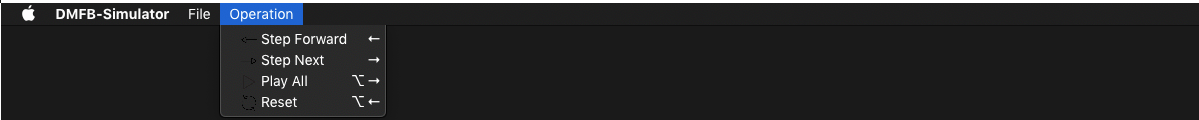
\includegraphics[width=15cm]{Img/menu.png}
				\caption{菜单栏}
			\end{figure}
		
			\begin{figure}[htbp]
				\centering
				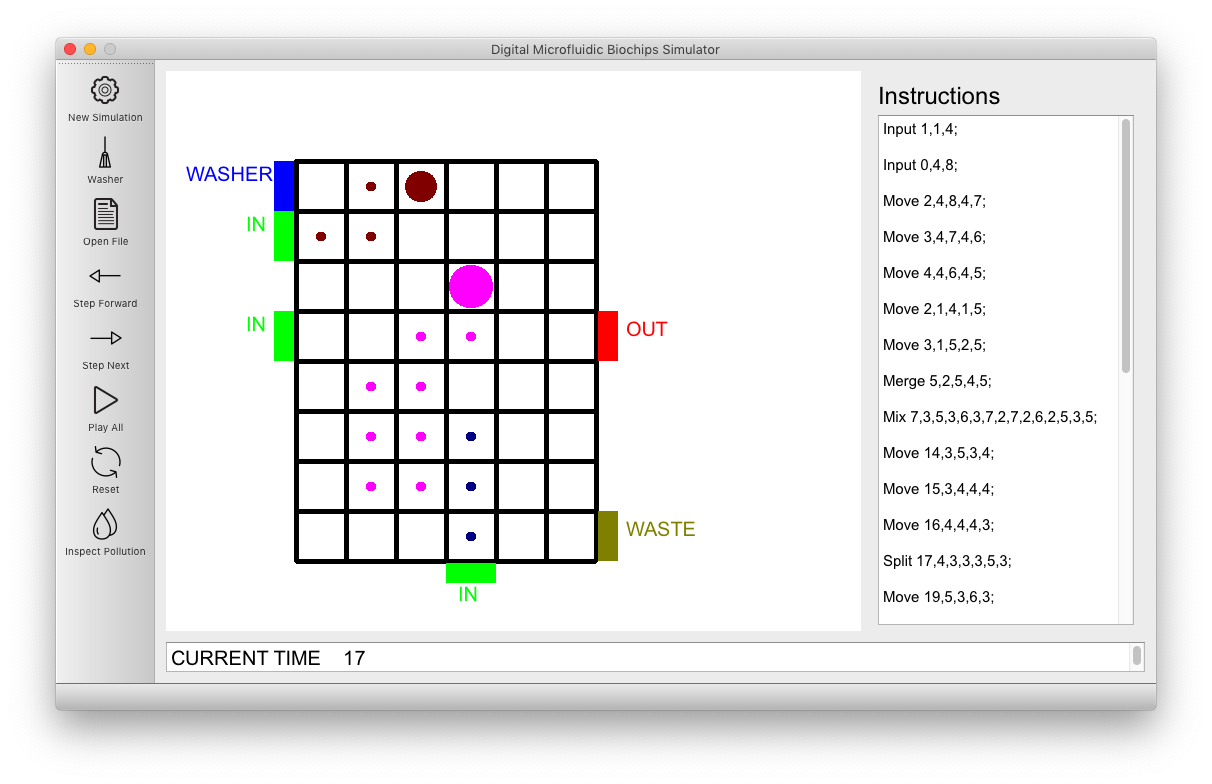
\includegraphics[width=15cm]{Img/main.png}
				\caption{主界面}
			\end{figure}
		
			\begin{figure}[htbp]
				\centering
				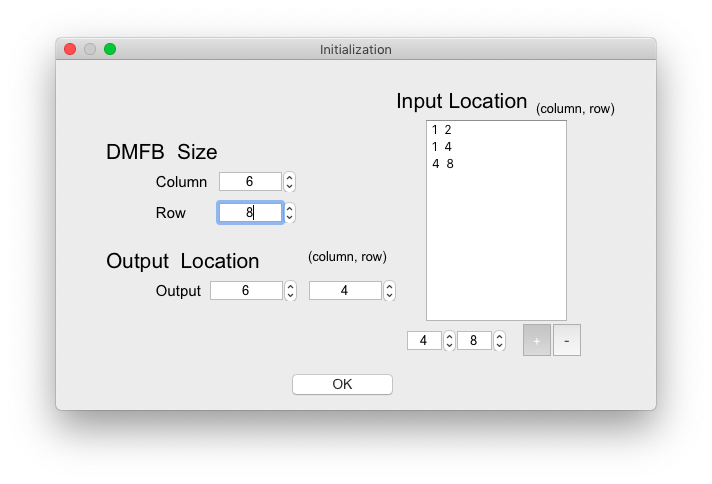
\includegraphics[width=15cm]{Img/init.png}
				\caption{芯片参数设置界面}
			\end{figure}
		
			\begin{figure}[htbp]
				\centering
				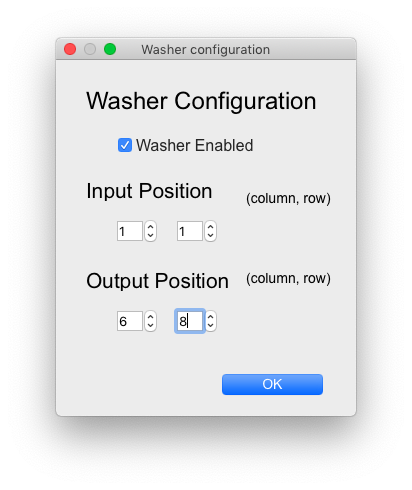
\includegraphics[width=5cm]{Img/washer.png}
				\caption{清洗液参数设置界面}
			\end{figure}
		\end{appendices}
\end{document} 
